% Options for packages loaded elsewhere
\PassOptionsToPackage{unicode}{hyperref}
\PassOptionsToPackage{hyphens}{url}
%
\documentclass[
  english,
  man,floatsintext]{apa6}
\usepackage{amsmath,amssymb}
\usepackage{lmodern}
\usepackage{ifxetex,ifluatex}
\ifnum 0\ifxetex 1\fi\ifluatex 1\fi=0 % if pdftex
  \usepackage[T1]{fontenc}
  \usepackage[utf8]{inputenc}
  \usepackage{textcomp} % provide euro and other symbols
\else % if luatex or xetex
  \usepackage{unicode-math}
  \defaultfontfeatures{Scale=MatchLowercase}
  \defaultfontfeatures[\rmfamily]{Ligatures=TeX,Scale=1}
\fi
% Use upquote if available, for straight quotes in verbatim environments
\IfFileExists{upquote.sty}{\usepackage{upquote}}{}
\IfFileExists{microtype.sty}{% use microtype if available
  \usepackage[]{microtype}
  \UseMicrotypeSet[protrusion]{basicmath} % disable protrusion for tt fonts
}{}
\makeatletter
\@ifundefined{KOMAClassName}{% if non-KOMA class
  \IfFileExists{parskip.sty}{%
    \usepackage{parskip}
  }{% else
    \setlength{\parindent}{0pt}
    \setlength{\parskip}{6pt plus 2pt minus 1pt}}
}{% if KOMA class
  \KOMAoptions{parskip=half}}
\makeatother
\usepackage{xcolor}
\IfFileExists{xurl.sty}{\usepackage{xurl}}{} % add URL line breaks if available
\IfFileExists{bookmark.sty}{\usepackage{bookmark}}{\usepackage{hyperref}}
\hypersetup{
  pdftitle={Does Double-Hard Debias Keep its Promises? - A Replication Study},
  pdfauthor={Kristina Kobrock1, Meike Korsten1, \& Sonja Börgerding1},
  pdflang={en-EN},
  pdfkeywords={keywords},
  hidelinks,
  pdfcreator={LaTeX via pandoc}}
\urlstyle{same} % disable monospaced font for URLs
\usepackage{graphicx}
\makeatletter
\def\maxwidth{\ifdim\Gin@nat@width>\linewidth\linewidth\else\Gin@nat@width\fi}
\def\maxheight{\ifdim\Gin@nat@height>\textheight\textheight\else\Gin@nat@height\fi}
\makeatother
% Scale images if necessary, so that they will not overflow the page
% margins by default, and it is still possible to overwrite the defaults
% using explicit options in \includegraphics[width, height, ...]{}
\setkeys{Gin}{width=\maxwidth,height=\maxheight,keepaspectratio}
% Set default figure placement to htbp
\makeatletter
\def\fps@figure{htbp}
\makeatother
\setlength{\emergencystretch}{3em} % prevent overfull lines
\providecommand{\tightlist}{%
  \setlength{\itemsep}{0pt}\setlength{\parskip}{0pt}}
\setcounter{secnumdepth}{-\maxdimen} % remove section numbering
% Make \paragraph and \subparagraph free-standing
\ifx\paragraph\undefined\else
  \let\oldparagraph\paragraph
  \renewcommand{\paragraph}[1]{\oldparagraph{#1}\mbox{}}
\fi
\ifx\subparagraph\undefined\else
  \let\oldsubparagraph\subparagraph
  \renewcommand{\subparagraph}[1]{\oldsubparagraph{#1}\mbox{}}
\fi
% Manuscript styling
\usepackage{upgreek}
\captionsetup{font=singlespacing,justification=justified}

% Table formatting
\usepackage{longtable}
\usepackage{lscape}
% \usepackage[counterclockwise]{rotating}   % Landscape page setup for large tables
\usepackage{multirow}		% Table styling
\usepackage{tabularx}		% Control Column width
\usepackage[flushleft]{threeparttable}	% Allows for three part tables with a specified notes section
\usepackage{threeparttablex}            % Lets threeparttable work with longtable

% Create new environments so endfloat can handle them
% \newenvironment{ltable}
%   {\begin{landscape}\begin{center}\begin{threeparttable}}
%   {\end{threeparttable}\end{center}\end{landscape}}
\newenvironment{lltable}{\begin{landscape}\begin{center}\begin{ThreePartTable}}{\end{ThreePartTable}\end{center}\end{landscape}}

% Enables adjusting longtable caption width to table width
% Solution found at http://golatex.de/longtable-mit-caption-so-breit-wie-die-tabelle-t15767.html
\makeatletter
\newcommand\LastLTentrywidth{1em}
\newlength\longtablewidth
\setlength{\longtablewidth}{1in}
\newcommand{\getlongtablewidth}{\begingroup \ifcsname LT@\roman{LT@tables}\endcsname \global\longtablewidth=0pt \renewcommand{\LT@entry}[2]{\global\advance\longtablewidth by ##2\relax\gdef\LastLTentrywidth{##2}}\@nameuse{LT@\roman{LT@tables}} \fi \endgroup}

% \setlength{\parindent}{0.5in}
% \setlength{\parskip}{0pt plus 0pt minus 0pt}

% \usepackage{etoolbox}
\makeatletter
\patchcmd{\HyOrg@maketitle}
  {\section{\normalfont\normalsize\abstractname}}
  {\section*{\normalfont\normalsize\abstractname}}
  {}{\typeout{Failed to patch abstract.}}
\patchcmd{\HyOrg@maketitle}
  {\section{\protect\normalfont{\@title}}}
  {\section*{\protect\normalfont{\@title}}}
  {}{\typeout{Failed to patch title.}}
\makeatother
\shorttitle{Replication: Wang et al. (2020)}
\keywords{keywords\newline\indent Word count: X}
\DeclareDelayedFloatFlavor{ThreePartTable}{table}
\DeclareDelayedFloatFlavor{lltable}{table}
\DeclareDelayedFloatFlavor*{longtable}{table}
\makeatletter
\renewcommand{\efloat@iwrite}[1]{\immediate\expandafter\protected@write\csname efloat@post#1\endcsname{}}
\makeatother
\usepackage{csquotes}
\ifxetex
  % Load polyglossia as late as possible: uses bidi with RTL langages (e.g. Hebrew, Arabic)
  \usepackage{polyglossia}
  \setmainlanguage[]{english}
\else
  \usepackage[main=english]{babel}
% get rid of language-specific shorthands (see #6817):
\let\LanguageShortHands\languageshorthands
\def\languageshorthands#1{}
\fi
\ifluatex
  \usepackage{selnolig}  % disable illegal ligatures
\fi
\newlength{\cslhangindent}
\setlength{\cslhangindent}{1.5em}
\newlength{\csllabelwidth}
\setlength{\csllabelwidth}{3em}
\newenvironment{CSLReferences}[2] % #1 hanging-ident, #2 entry spacing
 {% don't indent paragraphs
  \setlength{\parindent}{0pt}
  % turn on hanging indent if param 1 is 1
  \ifodd #1 \everypar{\setlength{\hangindent}{\cslhangindent}}\ignorespaces\fi
  % set entry spacing
  \ifnum #2 > 0
  \setlength{\parskip}{#2\baselineskip}
  \fi
 }%
 {}
\usepackage{calc}
\newcommand{\CSLBlock}[1]{#1\hfill\break}
\newcommand{\CSLLeftMargin}[1]{\parbox[t]{\csllabelwidth}{#1}}
\newcommand{\CSLRightInline}[1]{\parbox[t]{\linewidth - \csllabelwidth}{#1}\break}
\newcommand{\CSLIndent}[1]{\hspace{\cslhangindent}#1}

\title{Does Double-Hard Debias Keep its Promises? - A Replication Study}
\author{Kristina Kobrock\textsuperscript{1}, Meike Korsten\textsuperscript{1}, \& Sonja Börgerding\textsuperscript{1}}
\date{}


\affiliation{\vspace{0.5cm}\textsuperscript{1} University of Osnabrück}

\begin{document}
\maketitle

Just edit the text! There are several websites that help with (r)markdown, e.g.~\url{https://rmarkdown.rstudio.com/}.
If you don't want to edit directly, but rather comment use:
Cite using: Wang et al. (2020) said that\ldots{} or simply blablabla (Wang et al., 2020). References must be added to r-references.bib file.

\hypertarget{introduction}{%
\subsection{Introduction}\label{introduction}}

\begin{itemize}
\tightlist
\item
  shall we include an abstract?
  Recent research has shown that word embeddings derived from language corpora inherit human biases. The first seminal study on this topic was by Bolukbasi et al. (2016) who used the word analogy task developed by Mikolov et al. (2013) to prove that ``Man is to Computer Programmer as Woman is to Homemaker'' - a clearly gender biased analogical relation derived from a Google News embedding. Caliskan et al. (2017) complement this finding with a large study on human-like semantic biases in Natural Language Processing (NLP) tools. They have shown in more general that human biases as exhibited in psychological studies using, for example, the Implicit Association Test (IAT) are learned by NLP algorithms designed to construct meaningful word representations. According to Zhao et al. (2018) these biases propagate to downstream tasks. As pre-trained word embeddings are often used for a lot of more complex NLP tasks and architectures of our everyday life, the biased embeddings bear the risk of proliferating and strengthening existing stereotypes in human cultures.
\end{itemize}

\hypertarget{debiasing-embeddings}{%
\subsubsection{Debiasing Embeddings}\label{debiasing-embeddings}}

But how can the problem of biased embeddings be solved? Several researchers have proposed post-processing techniques or algorithm modifications that promise to ``debias'' the word embeddings obtained by algorithms like word2vec or GloVe (e.g. Bolukbasi, Chang, Zou, Saligrama, \& Kalai, 2016; Kaneko \& Bollegala, 2019; Zhao, Zhou, Li, Wang, \& Chang, 2018).
Bolukbasi et al. (2016) have developed an algorithm called Hard Debias that is based on the idea of removing (biased) gender directions from the embedding whilst preserving desired gender relations. For example, the encoded gender of the words ``king'' and ``queen'' is given by definition. So the relation between ``male'' and ``king'' and between ``female'' and ``queen'' is desired. On the other hand, words like ``nurse'' and ``doctor'' also tend to exhibit relations to a specific gender even though the words do not have a gender-specific meaning but can be used for all genders. The proposed Hard Debias algorithm first identifies a gender subspace of the embedding that best captures the bias. Then a neutralizing step ensures that gender neutral words (like ``nurse'' and ``doctor'') are indeed neutral, i.e.~zero, in the gender subspace. An equalizing step is then applied in order to ensure that useful relations apply to words from both genders and are not biased towards one gender anymore. For example, the word ``babysit'' should be equally distant from both ``she'' and ``he.''
Wang et al. (2020) build on Hard Debias in their newly proposed Double Hard Debias algorithm. The main idea is to not only remove the gender direction of the biased embedding, but also the frequency direction as it has been shown that word frequency has a significant impact on the geometry of the embedding space (e.g. Gong et al., 2018; Mu, Bhat, \& Viswanath, 2018, more on this later).

\hypertarget{motivation}{%
\subsubsection{Motivation}\label{motivation}}

In this project, we aimed to replicate the debiasing method presented by Wang et al. (2020) and to reproduce their experimental results as it is the most recent paper that proposes a post-processing technique for debiasing algorithms.
The reproduction of existing results is not only good practice in science, but it is also essential for gaining a deeper understanding on the methods used and it can help to validate existing results or to shed well-grounded doubt on them. Recent studies of reproducibility in the field of Computer Science (e.g. Collberg, Proebsting, \& Warren, 2015) and NLP (Belz, Agarwal, Shimorina, \& Reiter, 2021; Cohen et al., 2018; e.g. Fokkens et al., 2013; Mieskes, 2017) explain why reproducibility endeavours are often failing and shed light on the exact nature of the `reproducibility crisis' (term coined by e.g. Baker, 2015) in NLP research. Belz et al. (2021), for example, report that the community's interest in topics of reproducibility have risen even though reproduction attempts still tend to fail due to problems like missing data, missing code and incomplete documentation (see also Fokkens et al., 2013; Mieskes, Fort, Névéol, Grouin, \& Cohen, 2019).
This project aims to make a contribution to the increasing body of reproducibility and replication attempts in NLP research.

\hypertarget{implementation}{%
\subsection{Implementation}\label{implementation}}

\begin{itemize}
\tightlist
\item
  task description
\item
  explanation of model and training choices
\end{itemize}

\hypertarget{pilot-study-impact-of-word-frequency-meike}{%
\subsubsection{Pilot Study: Impact of Word Frequency (Meike)}\label{pilot-study-impact-of-word-frequency-meike}}

\hypertarget{datasets-and-preliminaries-sonja}{%
\subsubsection{Datasets and Preliminaries (Sonja)}\label{datasets-and-preliminaries-sonja}}

As dataset we used the pre-trained, 300-dimensional GloVe embedding used and provided via link on Github by Wang et al. (2020). Further they also provided several more datasets that were obtained through different debiasing methods, some applied during training, some after. The authors{]} used these datasets as baselines for the evaluation to compare the perfomance of their Double-Hard Debias method to. Lastly they also provide the embedding that is the reult of applying their Double-Hard Debias alogrithm to the original, non-debiased GloVe embedding. We included all of these embeddings in our evaluation to compore to the result of our implementation of Double-Hard Debias.

The original files included 300-dimensional embeddings for 322.636 words. To avoid large downloads we decided to open the files via URL, however this was not possible for the Double-Hard Debiased embedding obtained by Wang et al. (2020), therefor this embedding needs to be downloaded and open seperatly. From all the provided files we created for each embedding a vocabulary in form of a list, a dictionary mapping all words in the vocabulary to an ID and an embedding matrix that stores the 300-dimensional embedding of each word in the row corresponding to the ID of the word. During the pre-processing we restricted the vocabularies to the 50.000 most common words, which corresponds to the first 50.000 words in a GloVe embedding. At this point we also excluded any words that contain digits or special characters from our vocabularies. Both these actions follow the implementation provided by Wang et al. (2020), however the restriction to 50.000 words is not documented and apparently only happens in the code demonstrating the Double-Hard debiasing method for computational reasons. We adopted this restriction for computational reasons as well as the hope to remove some less frequent words such as names from our embedding to obtain more general results. However unlike the authors we did not specifically remove any non lower case words as the GloVe embedding is lower-cased by default and we also refrained from excluding all words longer than 20 characters.

We made use of a number of word sets provided by Wang et al. (2020). For the application of Hard Debias as proposed by Bolukbasi et al. (2016) we need sets of male and female words as well as a set of neutral words. We will later explain how we obtained the sets of gendered words based on determining the gender direction. For this we used the supplied ``definitional\_pairs,'' a word set including pairs such as ``he'' and ``she.'' To obtain the neutral set, we removed all words found in the files provided by Wang et al. (2020) from our vocabulary. These files included besides the aforementioned ``definitional\_pairs'' also ``equalize\_pairs,'' ``gender\_specific\_full,'' ``female\_word\_file'' and ``male\_word\_file'' in the assumption that all these files include definitionally gendered words that should not be included in the neutral set. However it stays unclear for some of these sets where Wang et al. (2020) obtained them, except for ``definitional\_pairs'' and ``equalize\_pairs'' which are the gender pairs and equality sets as suggested by Bolukbasi et al. (2016). Since the ``male\_word\_file'' and the ``female\_word\_file'' include pairs of corresponding words such as ``spokesman'' and ``spokeswoman'' or ``priest'' and ``nun'' we also created a set of pairs based on these two files to be used with the debiasing algorithm.

\hypertarget{hard-debias-kristina}{%
\subsubsection{Hard Debias (Kristina)}\label{hard-debias-kristina}}

The authors make use of the Hard Debias algorithm proposed by Bolukbasi et al. (2016). The paper at hand does not give much information on the exact implementation of Hard Debias used. The code uploaded to the authors' Github repository is not well documented, so we were not able to find the exact parts of the algorithm that should refer to the implementation of Hard Debias. That is why we sticked to the original paper from Bolukbasi et al. (2016) in order to re-implement Hard Debias.

The paper describes two steps: First, the gender direction (or, more generally, the subspace) has to be identified. This is achieved with the help of defining sets \(D_1, D_2, ..., D_n \subset W\) which consist of \emph{gender specific} words, i.e.~words which are associated with a gender by definition like \emph{girl, boy} or \emph{she, he}. These are the words that can help to identify the gender direction by capturing the concept \emph{female, male} in the embedding \(\{\vec{w}\in\mathbb{R}^d\}_{w\in W}\). Whereas in some simple implementations of Hard Debias, only one definitional pair might be used, (Bolukbasi, Chang, Zou, Saligrama, \& Kalai, 2016) suggest to compute the gender direction \(B\) across multiple pairs to more robustly estimate the bias. In our implementation we used the 10 word pairs suggested by Bolukbasi, Chang, Zou, Saligrama, and Kalai (2016) which were experimentally shown to agree with an intuitive concept of gender. For these 10 pairs the principal components (PCs) are calculated and the bias subspace \(B\) is made of the first \(k \geq 1\) rows of the decomposition SVD(\(C\)). According to Bolukbasi, Chang, Zou, Saligrama, and Kalai (2016), the first eigenvalue is significantly larger than the rest and so the top PC is hypothesized to capture the gender subspace. So \(k=1\) is chosen and our resulting gender subspace \(B\) is thus simply a direction. C is calculated in the following way: \[C:=\sum_{i=1}^n \sum_{w\in D_i}(\vec{w}-\mu_i)^T(\vec{w}-\mu_i)/|D_i|\] where \(\mu_i := \sum_{w\in D_i}\vec{w}/|D_i|\) are the means of the defining sets \(D_1, D_2, ..., D_n \subset W\).

As a second step Hard Debias neutralizes and equalizes the word embeddings. Neutralizing means to transform each word embedding \(\vec{w}\) such that every word \(w\in N\) has zero projection in the gender subspace. So for each word \(w\in N\) in a set of neutral words \(N \subseteq W\), we re-embed \(\vec{w}\): \[\vec{w}:=(\vec{w}-\vec{w}_B)/||\vec{w}-\vec{w}_B||\]. The equalize step ensures that desired analogical properties hold for both female and male words contained in the equality sets \(\mathcal{E}=\{E_1,E_2,...,E_m\}\) where each \(E_i \subseteq W\). For example, after debiasing we would like the embeddings of the pair \(E=\{grandmother, grandfather\}\) contained in the equality sets to be equidistant from the embedding of \emph{babysit} (Bolukbasi, Chang, Zou, Saligrama, \& Kalai, 2016). This is enforced by equating each set of words \(E\in \mathcal{E}\) outside of \(B\) to their simple average \(\nu:=\mu-\mu_B\) where \(\mu:=\sum_{w\in E}w/|E|\) before adjusting vectors so that they are unit length. So for each word \(w\in E\), \(\vec{w}\) is re-embedded to \[\vec{w}:=\nu+\sqrt{1-||\nu||^2}\frac{\vec{w}_B-\mu_B}{||\vec{w}_B-\mu_B||}\].

With the help of the original paper, we were successfully able to re-implement Hard Debias.

\hypertarget{double-hard-debias-meike}{%
\subsubsection{Double-Hard Debias (Meike)}\label{double-hard-debias-meike}}

As previously mentioned, the code provided by the authors' was rather unsatisfactory and superficial, which is why we choose to stick to the Pseudo code provided in the paper.

The Double-Hard Debias algorithm is set up such that two different directions are removed from the original embeddings. The first one being one supposedly encoding frequency information, the second one being the gender direction, as proposed by Bolukbasi et al. (Bolukbasi, Chang, Zou, Saligrama, \& Kalai, 2016).
In earlier work, Mu and Viswanath (2018) have shown, that further dimension reduction of word embeddings actually increases the linguistic regularities they capture. To do so, they first subtracted the common mean vector and then identified a few top principal components of the embedding space. After removing both of those components, the resulting word embeddings proof to serve as stronger representations. During the application of their algorithm, Mu and Viswanath (2018) noticed, that some the top PCA directions seemed to encode frequency to a significant degree.
Wang et al. (2020) base their algorithm mostly on those findings and also apply PCA to their algorithm, claiming that to be a feasible method to identify directions of the embedding space encoding word frequency.

The first part of the algorithm represents picking the frequency direction that shall ultimatly be removed from all embeddings.This is done in a trial-based set up on only the most biased words (500 male and female). Following Mu and Viswanath's (2018) work, the common mean vector is removed before PCA is applied.
In the Pseudocode presented, the authors depict the computation of the same number of principal components as the dimensionality that the embeddings in question have. In the provided code, on the other hand, they only compute the top 10 principal components, which is what we ultimately replicated.
For each of those PCs, the corresponding direction is removed, Hard Debias is applied on those projected embeddings, and performance of the resulting embeddings on the Neighborhood Metric, originally proposed by Gonen and Goldberg , is measured. This Metric and it's use is discussed in a more detailed manner in the evaluation part.
Then, the PC is identified that lead to the best performance on the Neighborhood Metric, here meaning resulting in least biased embeddings.
After identifying this component, it is picked out of all the PC candidates to\\
This direction, supposedly encoding frequency as well as gender information, is picked to proceed to the second part of the algorithm.
This second part deppicts the ``real'' debiasing of the full set of word embeddings, by first removing the recently identified direction, and subsequently applying Hard Debias.

\hypertarget{evaluation}{%
\subsection{Evaluation}\label{evaluation}}

\begin{itemize}
\tightlist
\item
  stick to the paper
\end{itemize}

\hypertarget{baselines-sonja}{%
\subsubsection{Baselines (Sonja)}\label{baselines-sonja}}

Following Wang et al. (2020) we used GloVe embeddings that were obtained using several different debiasing methods as baselines for our evaluation along with the original, non-debiased embedding.

original GloVe: The original, non-debiased GloVe embedding used and provided by Wang et al. (2020). It was obtained from training on the 2017 January dump of English Wikipedia.

GN-GloVe: Gender-Neutral GloVe embedding released by Zhao et al. (2018). This method restricts gender information in certain dimensions while neutralizing in the remaining dimensions.

GN-GloVe(a): A variant of the Gender-Neutral GloVe embedding obtained by Wang et al. (2020). It was created by excluding the gender dimensions from the GN-GloVe embedding in a try to completly remove gender.

GP-GloVe: Gender preserving GloVe embedding released by Kaneko and Bollegala (2019). This method attempts to remove stereotypical gender bias and preserve non-discriminative gender information.

GP-GN-GloVe: Gender preserving, Gender-Neutral GloVe embedding provided by Kaneko and Bollegala (2019). This is the result of applying gender preserving debiasing to an already debiased GN-GloVe embedding.

Hard-GloVe: Hard debiased GloVe embedding obtained by Wang et al. (2020) following the implementation of Bolukbasi et al. (2016). This method aims to debias neutral words while preserving the gender specific words.

Strong-Hard-GloVe: Strong-Hard debiased GloVe embedding obtained by Wang et al. (2020). A variant of Hard debias during which all words are debiased instead of only the neutral words.

Double-Hard-GloVe(Wang et al.): Double-Hard debiased GloVe embedding obtained by Wang et al. (2020). This is the result of applying their proposed Double-Hard Debias method to the original GloVe embedding.

Double-Hard-GloVe(replication): Double-Hard debiased GloVe embedding obtained by us. This is the result of applying our implementation of the Double-Hard Debias method to the original GloVe embedding.

\hypertarget{evaluation-of-debiasing-performance}{%
\subsubsection{Evaluation of Debiasing Performance}\label{evaluation-of-debiasing-performance}}

\hypertarget{debiasing-in-downstream-applications}{%
\subsubsection{Debiasing in Downstream Applications}\label{debiasing-in-downstream-applications}}

\hypertarget{coreference-resolution-meike}{%
\paragraph{Coreference Resolution (Meike)}\label{coreference-resolution-meike}}

\begin{itemize}
\tightlist
\item
  no replication possible, no code provided
\end{itemize}

\hypertarget{debiasing-at-embedding-level}{%
\subsubsection{Debiasing at Embedding Level}\label{debiasing-at-embedding-level}}

\hypertarget{the-word-embeddings-association-test-weat-sonja}{%
\paragraph{The Word Embeddings Association Test (WEAT) (Sonja)}\label{the-word-embeddings-association-test-weat-sonja}}

\begin{table}

\caption{(\#tab:table 1)WEAT Test}
\centering
\begin{tabular}[t]{l|r|r|r|r|r|r}
\hline
X & C...F..d & C...F..p & M...A..d & M...A..p & S...A..d & S...A..p\\
\hline
original GloVe & 1.805996 & 0.0001524 & 0.6885951 & 0.0850657 & 1.1298693 & 0.0119380\\
\hline
Double-Hard-GloVe (Wang et al.) & 1.531301 & 0.0010940 & -0.5625492 & 0.8692854 & -0.6502705 & 0.9027524\\
\hline
Double-Hard-GloVe (replication) & 1.529532 & 0.0011171 & -0.6895229 & 0.9160087 & -0.9418647 & 0.9708258\\
\hline
GN-Glove & 1.821105 & 0.0001351 & -0.2563579 & 0.6963340 & 1.0689540 & 0.0162131\\
\hline
GN-Glove(a) & 1.755476 & 0.0002232 & 0.5030034 & 0.1584799 & 0.8797335 & 0.0395316\\
\hline
GP-GloVe & 1.805885 & 0.0001498 & 1.2085292 & 0.0078522 & 1.1064400 & 0.0131905\\
\hline
GP-GN-GloVe & 1.797431 & 0.0001750 & -0.0126418 & 0.5079182 & 0.8460069 & 0.0453070\\
\hline
Hard-GloVe & 1.546646 & 0.0010009 & -0.9826043 & 0.9751140 & -0.5383765 & 0.8592254\\
\hline
Strong-Hard-GloVe & 1.546646 & 0.0009967 & -0.9856814 & 0.9754177 & -0.5471175 & 0.8625488\\
\hline
\end{tabular}
\end{table}

\hypertarget{neighborhood-metric-meike}{%
\paragraph{Neighborhood Metric (Meike)}\label{neighborhood-metric-meike}}

\begin{itemize}
\tightlist
\item
  discuss that this is shady in the discussion part
\end{itemize}

\begin{table}

\caption{(\#tab:table 2)Neighborhood Metric Clustering Accuracy}
\centering
\begin{tabular}[t]{l|r|r|r}
\hline
X & Top.100 & Top.500 & Top.1000\\
\hline
original GloVe & 1.000 & 1.000 & 1.0000\\
\hline
Double-Hard-GloVe (Wang et al.) & 0.545 & 0.565 & 0.5800\\
\hline
Double-Hard-GloVe (replication) & 0.525 & 0.506 & 0.5370\\
\hline
GN-Glove & 1.000 & 0.999 & 0.9990\\
\hline
GN-Glove(a) & 1.000 & 0.997 & 0.9835\\
\hline
GP-GloVe & 1.000 & 1.000 & 1.0000\\
\hline
GP-GN-GloVe & 1.000 & 0.998 & 0.9980\\
\hline
Hard-GloVe & 0.510 & 0.517 & 0.5030\\
\hline
Strong-Hard-GloVe & 0.510 & 0.518 & 0.5025\\
\hline
\end{tabular}
\end{table}

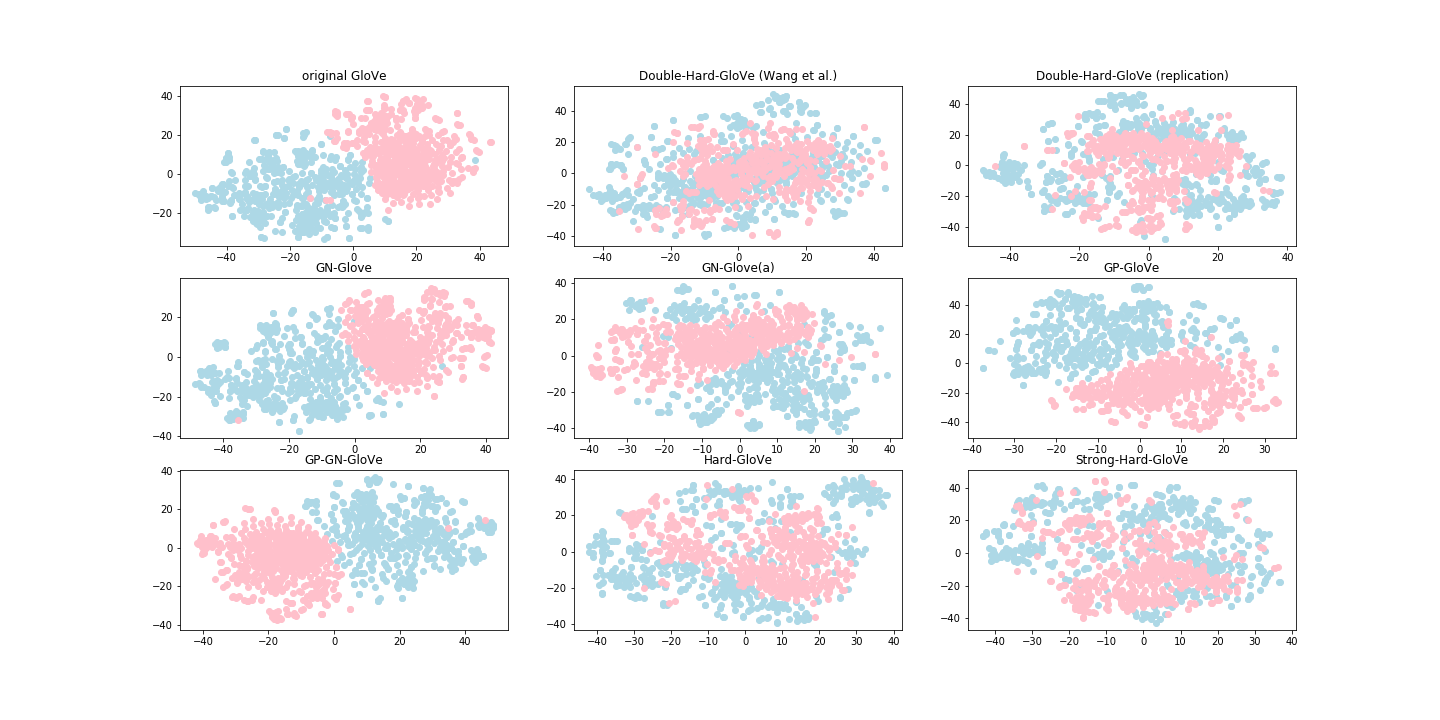
\includegraphics{evaluation_results/results_tsne.png}

\hypertarget{analysis-of-retaining-word-semantics-kristina}{%
\subsubsection{Analysis of Retaining Word Semantics (Kristina)}\label{analysis-of-retaining-word-semantics-kristina}}

One of the most important properties of embeddings is that they represent meaningful word semantics. In this section it is tested whether the debiased embeddings still have this property.

\hypertarget{word-analogy-kristina}{%
\paragraph{Word Analogy (Kristina)}\label{word-analogy-kristina}}

The word analogy task was introduced by Mikolov et al. (2013). The task is to find the word D such that ``A is to B as C is to D.'' One example for an unbiased analogy is: ``Man is to King as Woman is to Queen'' whereas a biased analogy would be: ``Man is to Computer Programmer as Woman is to Homemaker'' (Bolukbasi, Chang, Zou, Saligrama, \& Kalai, 2016). The debiased embeddings are evaluated on two word analogy test sets: the MSR (Mikolov, Yih, \& Zweig, 2013) and the Google word analogy task (Mikolov, Chen, Corrado, \& Dean, 2013) in order to find out whether they preserve desired unbiased analogies.

The MSR word analogy dataset contains 8000 syntactic questions in the form presented above. The missing word D is computed by maximizing the cosine similarity between D and C - A + B. The evaluation metric is the percentage of correctly answered questions (see Wang et al., 2020).

The Google word analogy dataset contains 19.544 (\textbf{Total}) questions, 8.869 of which are semantic (\textbf{Sem}) and 10.675 are syntactic (\textbf{Syn}) questions.

\begin{table}

\caption{(\#tab:tables 3 and 4)MSR Word Analogy Task}
\centering
\begin{tabular}[t]{l|r}
\hline
X & MSR\\
\hline
original GloVe & 0.5440213\\
\hline
Double-Hard-GloVe (Wang et al.) & 0.4240000\\
\hline
Double-Hard-GloVe (replication) & 0.6212121\\
\hline
GN-Glove & 0.5171990\\
\hline
GN-Glove(a) & 0.5071663\\
\hline
GP-GloVe & 0.5161753\\
\hline
GP-GN-GloVe & 0.5198608\\
\hline
Hard-GloVe & 0.6257166\\
\hline
Strong-Hard-GloVe & 0.6214169\\
\hline
\end{tabular}
\end{table}

\begin{table}

\caption{(\#tab:tables 3 and 4)Google Word Analogy Task}
\centering
\begin{tabular}[t]{l|r|r|r}
\hline
X & Sem & Syn & Total\\
\hline
original GloVe & 0.8014096 & 0.5569170 & 0.6389759\\
\hline
Double-Hard-GloVe (Wang et al.) & 0.7135838 & 0.4799063 & 0.5667098\\
\hline
Double-Hard-GloVe (replication) & 0.8020315 & 0.6655147 & 0.7113338\\
\hline
GN-Glove & 0.7597430 & 0.5466541 & 0.6181730\\
\hline
GN-Glove(a) & 0.7589138 & 0.5425699 & 0.6151812\\
\hline
GP-GloVe & 0.8192371 & 0.5541942 & 0.6431504\\
\hline
GP-GN-GloVe & 0.7574627 & 0.5667609 & 0.6307660\\
\hline
Hard-GloVe & 0.7999585 & 0.6610116 & 0.7076463\\
\hline
Strong-Hard-GloVe & 0.7674129 & 0.6573463 & 0.6942879\\
\hline
\end{tabular}
\end{table}

\hypertarget{concept-categorization-sonja}{%
\paragraph{Concept Categorization (Sonja)}\label{concept-categorization-sonja}}

\hypertarget{discussion}{%
\subsection{Discussion}\label{discussion}}

\begin{itemize}
\tightlist
\item
  analysis of results and evaluation of performance evaluation
\item
  ablation studies (not applicable)
\item
  discuss the results and what could be (partly) replicated and what not
\end{itemize}

\hypertarget{conclusion}{%
\subsection{Conclusion}\label{conclusion}}

\newpage

\hypertarget{references}{%
\section{References}\label{references}}

\begingroup
\setlength{\parindent}{-0.5in}
\setlength{\leftskip}{0.5in}

\hypertarget{refs}{}
\begin{CSLReferences}{1}{0}
\leavevmode\hypertarget{ref-baker_2015}{}%
Baker, M. (2015). Reproducibility crisis: Blame it on the antibodies. \emph{Nature}, \emph{521}(7552), 274--276. https://doi.org/\url{https://doi.org/10.1038/521274a}

\leavevmode\hypertarget{ref-belz_2021}{}%
Belz, A., Agarwal, S., Shimorina, A., \& Reiter, E. (2021). A systematic review of reproducibility research in natural language processing. Retrieved from \url{http://arxiv.org/abs/2103.07929}

\leavevmode\hypertarget{ref-bolukbasi_2016}{}%
Bolukbasi, T., Chang, K.-W., Zou, J. Y., Saligrama, V., \& Kalai, A. (2016). Man is to computer programmer as woman is to homemaker? Debiasing word embeddings. \emph{CoRR}, \emph{abs/1607.06520}. Retrieved from \url{http://arxiv.org/abs/1607.06520}

\leavevmode\hypertarget{ref-caliskan_2017}{}%
Caliskan, A., Bryson, J. J., \& Narayanan, A. (2017). Semantics derived automatically from language corpora contain human-like biases. \emph{Science}, \emph{356}(6334), 183--186. \url{https://doi.org/10.1126/science.aal4230}

\leavevmode\hypertarget{ref-cohen_2018}{}%
Cohen, K. B., Xia, J., Zweigenbaum, P., Callahan, T., Hargraves, O., Goss, F., \ldots{} Hunter, L. E. (2018). Three dimensions of reproducibility in natural language processing. In \emph{Proceedings of the eleventh international conference on language resources and evaluation ({LREC} 2018)}. Miyazaki, Japan: European Language Resources Association (ELRA). Retrieved from \url{https://www.aclweb.org/anthology/L18-1025}

\leavevmode\hypertarget{ref-collberg_2015}{}%
Collberg, C., Proebsting, T., \& Warren, A. M. (2015). Repeatability and benefaction in computer systems research. studie. Retrieved from \url{http://reproducibility.cs.arizona.edu/v2/RepeatabilityTR.pdf}

\leavevmode\hypertarget{ref-fokkens_2013}{}%
Fokkens, A., Erp, M. van, Postma, M., Pedersen, T., Vossen, P., \& Freire, N. (2013). Offspring from reproduction problems: What replication failure teaches us. In \emph{Proceedings of the 51st annual meeting of the association for computational linguistics (volume 1: Long papers)} (pp. 1691--1701). Sofia, Bulgaria: Association for Computational Linguistics. Retrieved from \url{https://www.aclweb.org/anthology/P13-1166}

\leavevmode\hypertarget{ref-gong_2018}{}%
Gong, C., He, D., Tan, X., Qin, T., Wang, L., \& Liu, T.-Y. (2018). FRAGE: Frequency-agnostic word representation. In S. Bengio, H. Wallach, H. Larochelle, K. Grauman, N. Cesa-Bianchi, \& R. Garnett (Eds.), \emph{Advances in neural information processing systems} (Vol. 31). Curran Associates, Inc. Retrieved from \url{https://proceedings.neurips.cc/paper/2018/file/e555ebe0ce426f7f9b2bef0706315e0c-Paper.pdf}

\leavevmode\hypertarget{ref-kaneko_2019}{}%
Kaneko, M., \& Bollegala, D. (2019). Gender-preserving debiasing for pre-trained word embeddings. In \emph{Proceedings of the 57th annual meeting of the association for computational linguistics} (pp. 1641--1650). Florence, Italy: Association for Computational Linguistics. \url{https://doi.org/10.18653/v1/P19-1160}

\leavevmode\hypertarget{ref-mieskes_2017}{}%
Mieskes, M. (2017). A quantitative study of data in the {NLP} community. In \emph{Proceedings of the first {ACL} workshop on ethics in natural language processing} (pp. 23--29). Valencia, Spain: Association for Computational Linguistics. \url{https://doi.org/10.18653/v1/W17-1603}

\leavevmode\hypertarget{ref-mieskes_2019}{}%
Mieskes, M., Fort, K., Névéol, A., Grouin, C., \& Cohen, K. B. (2019). {NLP Community Perspectives on Replicability.} In \emph{{Recent Advances in Natural Language Processing}}. Varna, Bulgaria. Retrieved from \url{https://hal.archives-ouvertes.fr/hal-02282794}

\leavevmode\hypertarget{ref-mikolov2013Google}{}%
Mikolov, T., Chen, K., Corrado, G., \& Dean, J. (2013). Efficient estimation of word representations in vector space. Retrieved from \url{http://arxiv.org/abs/1301.3781}

\leavevmode\hypertarget{ref-mikolov2013MSR}{}%
Mikolov, T., Yih, W., \& Zweig, G. (2013). Linguistic regularities in continuous space word representations. In \emph{Proceedings of the 2013 conference of the north {A}merican chapter of the association for computational linguistics: Human language technologies} (pp. 746--751). Atlanta, Georgia: Association for Computational Linguistics. Retrieved from \url{https://www.aclweb.org/anthology/N13-1090}

\leavevmode\hypertarget{ref-mu_2018}{}%
Mu, J., Bhat, S., \& Viswanath, P. (2018). All-but-the-top: Simple and effective postprocessing for word representations. Retrieved from \url{http://arxiv.org/abs/1702.01417}

\leavevmode\hypertarget{ref-wang_2020}{}%
Wang, T., Lin, X. V., Rajani, N. F., McCann, B., Ordonez, V., \& Xiong, C. (2020). Double-hard debias: Tailoring word embeddings for gender bias mitigation. In \emph{Association for computational linguistics (ACL)}.

\leavevmode\hypertarget{ref-zhao_2018a}{}%
Zhao, J., Wang, T., Yatskar, M., Ordonez, V., \& Chang, K.-W. (2018). Gender bias in coreference resolution: Evaluation and debiasing methods (pp. 15--20). \url{https://doi.org/10.18653/v1/N18-2003}

\leavevmode\hypertarget{ref-zhao_2018b}{}%
Zhao, J., Zhou, Y., Li, Z., Wang, W., \& Chang, K.-W. (2018). Learning gender-neutral word embeddings. In \emph{Proceedings of the 2018 conference on empirical methods in natural language processing} (pp. 4847--4853). Brussels, Belgium: Association for Computational Linguistics. \url{https://doi.org/10.18653/v1/D18-1521}

\end{CSLReferences}

\endgroup


\end{document}
